\graphicspath{{./fig_stokes2nd/}}

\subsection{振動平板による流れ: Stokesの第二問題}

\subsubsection{目的}
本例題は,無限に広い平板が粘性流体の中で振動するときに,引き起こされる流体の運動\cite{hino:74:fd, imai:73}(Stokesの第二問題)について,CBCソルバーの動作検証と予測精度を明らかにする.なお,本例題は,組込例題「Rect」クラスの2次元を用いる.

\subsubsection{問題の定義と厳密解}
いま,無限に広い平板が無限に広がっている粘性流体の中で自分自身に平行に単振動をしている場合を考える.
平板の振動方向に$x$軸をとり,平板自身は$xz$平面内で運動するものとすれば,それによって引き起こされる流体の運動は$x$軸に平行である.

Navier-Stokesの方程式から導かれる,この場合の基礎方程式は,
\begin{equation}
\frac{\partial u}{\partial t} = \nu \frac{\partial^2 u}{\partial y^2},\mbox{  } y>0
\label{eq:kiso}
\end{equation}
となる(平板の片側の半無限の領域$y>0$を考える).

境界条件は,

\begin{equation}
\begin{array}{lcl}
y \rightarrow \infty & : & u \rightarrow 0 \\
y = 0 & : & u = U cos (\omega t)
\end{array}
\label{eq:kyokai}
\end{equation}

具体的には
境界条件$y=0$の速度を

\begin{equation}
y=0\mbox{ }:\mbox{ }u=U e^{i \omega t}
\label{eq:kyokai_e}
\end{equation}

と置き換え,得られた結果の実数部
$Re(u)$をとればよい.

$u$は,$y$の関数と考えられるので,$u$の解の形として,

\begin{equation*}
u=f(y)e^{i \omega t}
\end{equation*}

を求めることにする.これを\textbf{式(\ref{eq:kiso})}に代入すると,

\begin{equation*}
\frac{d^2 f}{dy^2}=\frac{i \omega}{\nu}f
\end{equation*}

の二階常微分方程式が求まり,その一般解は,

\begin{equation*}
f=Ae^{\lambda y} + B e^{-\lambda y}, \mbox{  }A, \, B\mbox{は任意定数}
\end{equation*}

の形に与えられる.ただし,

\begin{equation*}
\lambda=\sqrt{\frac{i \omega}{\nu}}
=\sqrt{i}\sqrt{\frac{\omega}{\nu}}
=\frac{1+i}{\sqrt{2}}\sqrt{\frac{\omega}{\nu}}
=(1+i)\,k, \mbox{ ここで}
k=\sqrt{\frac{\omega}{2\nu}}
\end{equation*}

である.$y \rightarrow \infty$に対して,$e^{\lambda y} \rightarrow \infty$であるから,境界条件(\ref{eq:kyokai})から$A=0$.また境界条件(\ref{eq:kyokai_e})から,$B=U$が得られる.したがって,

\begin{eqnarray*}
u & = & Re \left(f(y)e^{i \omega t}\right) 
=Re\left(U e^{-\lambda y} e^{i\omega t }\right)
= Re \left(U e^{-ky}e^{i(\omega t - ky)}\right) \nonumber\\
 & = & U e^{-ky}cos (\omega t - ky)
\end{eqnarray*}

が求める解である.これは$y$方向に伝わる減衰性の正弦波で,その位相速度は,

\begin{equation*}
c=\frac{\omega}{k}=\sqrt{2 \omega \nu}
\end{equation*}

で与えられる.波数および減衰定数はともに$k=\sqrt{\omega/2\nu}$である.したがって,1波長$2 \pi/k$進む間に振幅は
$e^{-2\pi}\simeq0.002$倍に減衰してしまうので,実際上は波動的な性格は現れない.

いま,

\begin{equation}
\delta = \frac{1}{k} = \sqrt{\frac{2 \nu}{\omega}}
\label{eq:delta}
\end{equation}

とおけば,$\delta$は振幅が$1/e\simeq0.36788$倍に減衰する距離を表す.
平板の振動によって流体は揺り動かされるが,その動く距離はだいたい$\delta$の
厚さの層に限られていると考えられる.
すなわち,振動平板には厚さ$\delta$の境界層が付随すると考えられる.
この境界層の厚さは,粘性が小さいほど,また平板の振動数が大きいほど薄くなる.

\textbf{図\ref{fig:stokes_exact}}に,厳密解$u/U=e^{-ky}cos(\omega t-ky)$を$\omega t=0.5\pi, \, \pi, \, 1.5\pi, 2.0\pi$に対してプロットした.
文献\cite{hino:74:fd}との比較のため,縦軸には,無次元長さ$(y_1=)\sqrt{2}ky$をとっている.なお,減衰の様子が明確になるように$\cos(ky)$を,また境界層厚み$\delta = 1/k$を重ねてプロットしている.

\begin{figure}[htbp]
\begin{center}
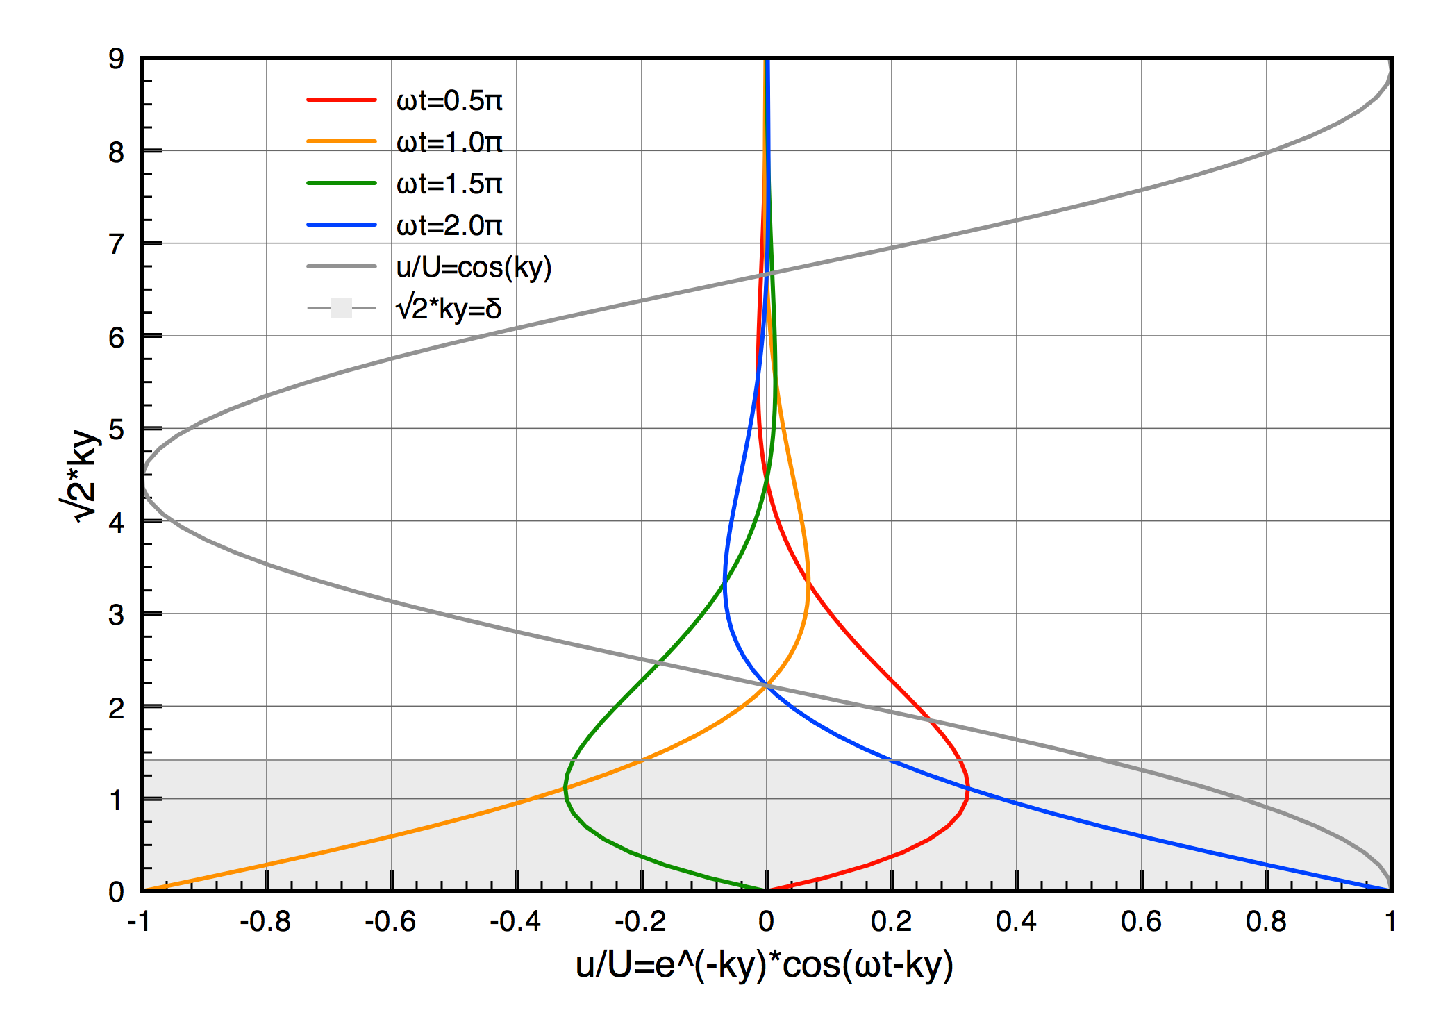
\includegraphics[width=14cm]{stokes_exact_cos1.eps}
\end{center}
\caption{Stokesの振動流の厳密解}
\label{fig:stokes_exact}
\end{figure}

%
\subsubsection{計算問題の準備}
作動流体として水($\nu=1.004 \times 10^{-6}[m^2/s]$),
振動数を$f=0.05[Hz]$,角振動数を$\omega=2\pi f=0.314[rad/s]$と考えると,
\textbf{式(\ref{eq:delta})}から,境界層厚さ,$\delta$は,2.5[mm]程度と算出される.
本計算では,$y$軸方向は,さらに減衰するまで,具体的には,10$\delta=2.5$[cm]以上の領域を,時間的には2周期,$\omega t=4\pi$まで計算することとした.

%
\subsubsection{計算領域と計算パラメータ}
「Rect」クラスの解析モデルは,全体領域を「Domain\_Info」タグで,2次元,3次元の別を「Intrinsic\_Example」タグで指定する.コンフィギュレーションファイル内の組込モデル名は,以下に示すように「Rectangular」である.\\
\hspace{1cm} $<$Param dtype="STRING" name="Example" value="Rectangular"/$>$\\

計算領域は,$-1.28\times 10^{-2}$[m]$\leq x \leq1.28\times 10^{-2}$[m],$0.00$[m]$\leq y \leq2.80\times 10^{-2}$[m],$-0.5\times 10^{-4}$[m]$\leq z \leq2.5\times 10^{-4}$[m],格子間隔は,$1.00\times 10^{-4}$[m],格子数を$256\times280\times3$として$z$方向に3層をとる,実質的2次元空間である.
総セル数は,215,040.$y=0$のY\_minus境界を振動面とみなし,$z$方向には,周期境界条件を設けている.

計算に用いた物性値を\textbf{表\ref{table:stokes_bussei}}に示す.物性値は,常温の水の値を使用した.

\begin{table}[htbp]
\begin{center}
\caption{計算に用いた物性}
\label{table:stokes_bussei}
\begin{tabular}{lccl}
\toprule
物性	&&物性値 &[単位]\\
\hline
動粘性係数& $\nu$&$1.004\times 10^{-6}$ & [m$^2$/s] \\
\bottomrule
\end{tabular}
\end{center}
\end{table}

計算に用いた外部境界条件を\textbf{表\ref{table:stokes bci}}に示す.

\begin{table}[hdpt]
%\small
\caption{計算に用いた境界条件}
\label{table:stokes bci}
\begin{center}
\begin{tabular}{lll}
\toprule
位置&タグ	&条件 	\\
\hline
 X\_minus, \, X\_plus&Periodic & Simple \\
 Y\_minus&Specified\_Velocity & Harmonic \\
 Y\_plus&Traction\_Free &\\
Z\_minus, \, Z\_plus& Periodic & Simple \\
\bottomrule
\end{tabular}
\end{center}
\end{table}

CBCに組み込まれているHarmonic運動は,次式で表される.
\begin{equation}
u=U \sin(2\pi f t + \phi)+b
\end{equation}
本計算では,以下のように設定した.
\begin{eqnarray}
U & = & 1.8\times 10^{-2} \mbox{[m/s]}\nonumber\\
f & = & 0.05\mbox{[Hz]}\nonumber\\
\phi & = & 0.5 \pi\mbox{[radian]}\nonumber\\
b & = & 0.0\mbox{[m/s]}
\end{eqnarray}  

\subsubsection{計算環境}
本計算に利用した計算機環境とソフトウェアを\textbf{表\ref{tbl: stokes env}}に示す.

\begin{table}[htdp]
\small
\caption{計算機環境および利用ソフトウェア}
\begin{center}
\begin{tabular}{ll}\toprule
Computer & eX. COMPUTER エアロストリーム RA7J-G23/S\\
CPU & Intel Core i7-950 (4 Cores/CPU)$\times$2\\
Clock & 3.07 GHz\\
Memory & 12GB \\
Cache & 8 MB\\
OS & Linux kernel 2.6.32-25-generic, ubuntu 10.04.1\\ \hline
MPI & OpenMPI 1.4.3\\
V-Sphere & ver. 1.8.4\\
CBC & ver. 1.4.6\\
FlowBase & ver. 2.4.3\\ \hline
Compiler & Intel Compiler Composer XE(12.0) 2011.3.174 C++/Fortran\\
Compile Option & -O3\\
\bottomrule
\end{tabular}
\end{center}
\label{tbl: stokes env}
\end{table}

\subsubsection{計算方法}
計算は,Navier-Stokes方程式を基礎方程式とし,時間積分は一次精度Euler陽解法,解法アルゴリズムにはFractional Step法を用いた.また,対流項の計算スキームには,三次精度MUSCLスキームを用いた.

時間積分幅の決定に,CFL\_Reference\_Velocityを使用し,クーラン数を0.2と指定した.また,計算時間は,$\omega t=4\pi$,$\omega=0.1\pi$より,$t=40$[sec]とした.

代表長さは$L=1.28\times 10^{-2}$[m],代表速度は$U=1.8\times 10^{-2}$[m/s]とした,代表時間は$t_0=7.1\dot{1}\times 10^{-1}$[sec],レイノルズ数はRe=230となる,

\paragraph{サンプリングの指定}
速度の値は,$x=0, \, z=0$上の$y=0 \sim y_{max}$の範囲を128分割してサンプリングする.サンプリング時間間隔は,$\omega t=0.5\pi$,$t=5$[sec]=7.03125[-]とした.

\subsubsection{計算結果と厳密解の比較}
\textbf{図\ref{fig:stokes_hikaku}}に,$\omega t=2.5\pi, \, 3.0\pi, \, 3.5\pi, \, 4.0\pi$におけるCBCによる計算結果と,$\omega t=0.5\pi, \, 1.0\pi, \, 1.5\pi, \, 2.0\pi$における厳密解を比較する.

なお,sampling.log結果ファイルの出力には,無次元を指定した.速度の無次元化された値はそのまま使用できるが,長さの無次元値には注意が必要である.CBCでは,一般的な無次元化,
\[
y_0=\frac{y}{L}
\]
を採用しているため,ファイルには$y_0$の値が出力される.
本例題では,文献\cite{hino:74:fd}および\textbf{図\ref{fig:stokes_exact}}との整合性のため,
\[
y_1=\sqrt{2}ky
\]
による無次元化を使用するため,$y_0\rightarrow y_1$の変換が必要である.
\[
y_1=\sqrt{2}ky=\sqrt{2}kLy_0=\sqrt{2}\sqrt{\frac{\omega}{2\nu}}Ly_0=\sqrt{\frac{2\pi f}{\nu}}Ly_0=7.16\times y_0
\]

\begin{figure}[htbp]
\begin{center}
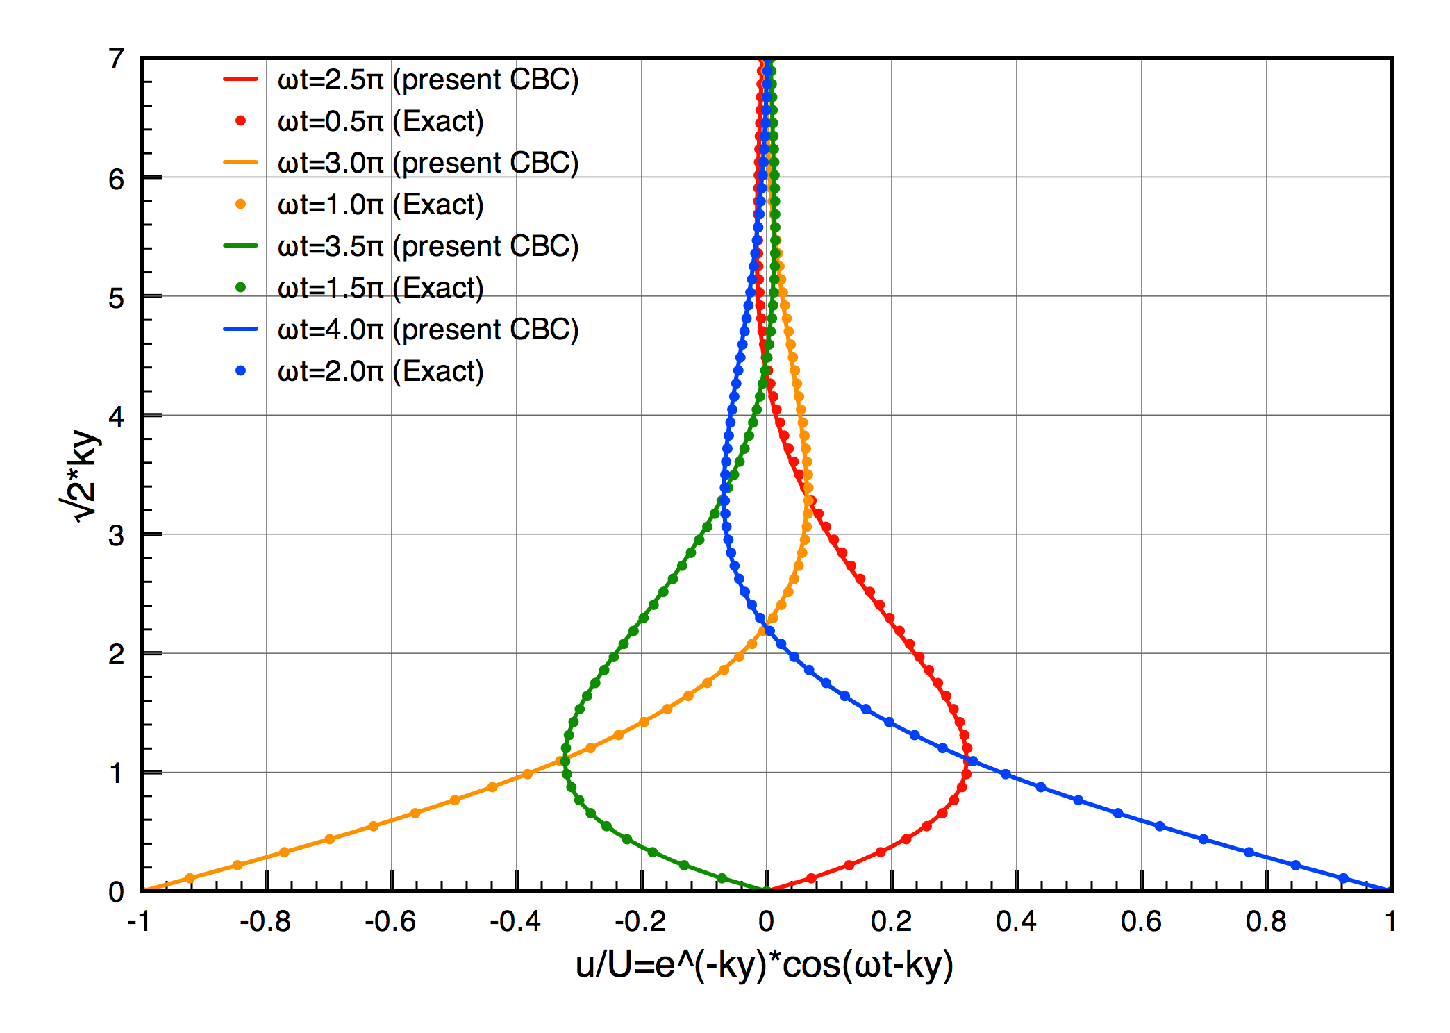
\includegraphics[width=14cm]{13stokes.eps}
\end{center}
\caption{Stokesの振動流の計算結果と厳密解の比較(計算2周期目)}
\label{fig:stokes_hikaku}
\end{figure}

CBCの計算結果は厳密解と非常によく一致しているように見える.しかしながら$\omega t=2,5\pi, \, 3.0\pi$では,
$\sqrt{2}ky\simeq 3$あたりで,僅かにずれている様子がわかる.

$\omega t=0.5\pi \sim 2.0\pi$ではCBCのずれはより大きい.
\textbf{図\ref{fig:stokes_hikaku1}}に,計算1周期目のCBCの結果と厳密解の比較を示す.

また,
CBCの計算結果の厳密解からの誤差を\textbf{図\ref{fig:stokes_error}}に示す.
時間を追うに従い,誤差が減少している様子がわかる.
1周期目(実線)では,$\omega t=0.5\pi$の最大誤差が厳密解の18.7\%,
2周期目(点線)では,$\omega t=2.5\pi$の最大誤差が厳密解の3.8\%,
$\omega t=4.0\pi$の最大誤差が厳密解の2.4\%である.
これらの誤差は,時間積分を一次精度Euler陽解法で行っていることが理由として考えられる.今後の課題として,時間積分の精度を上げて確認する予定である.

\begin{figure}[htbp]
\begin{center}
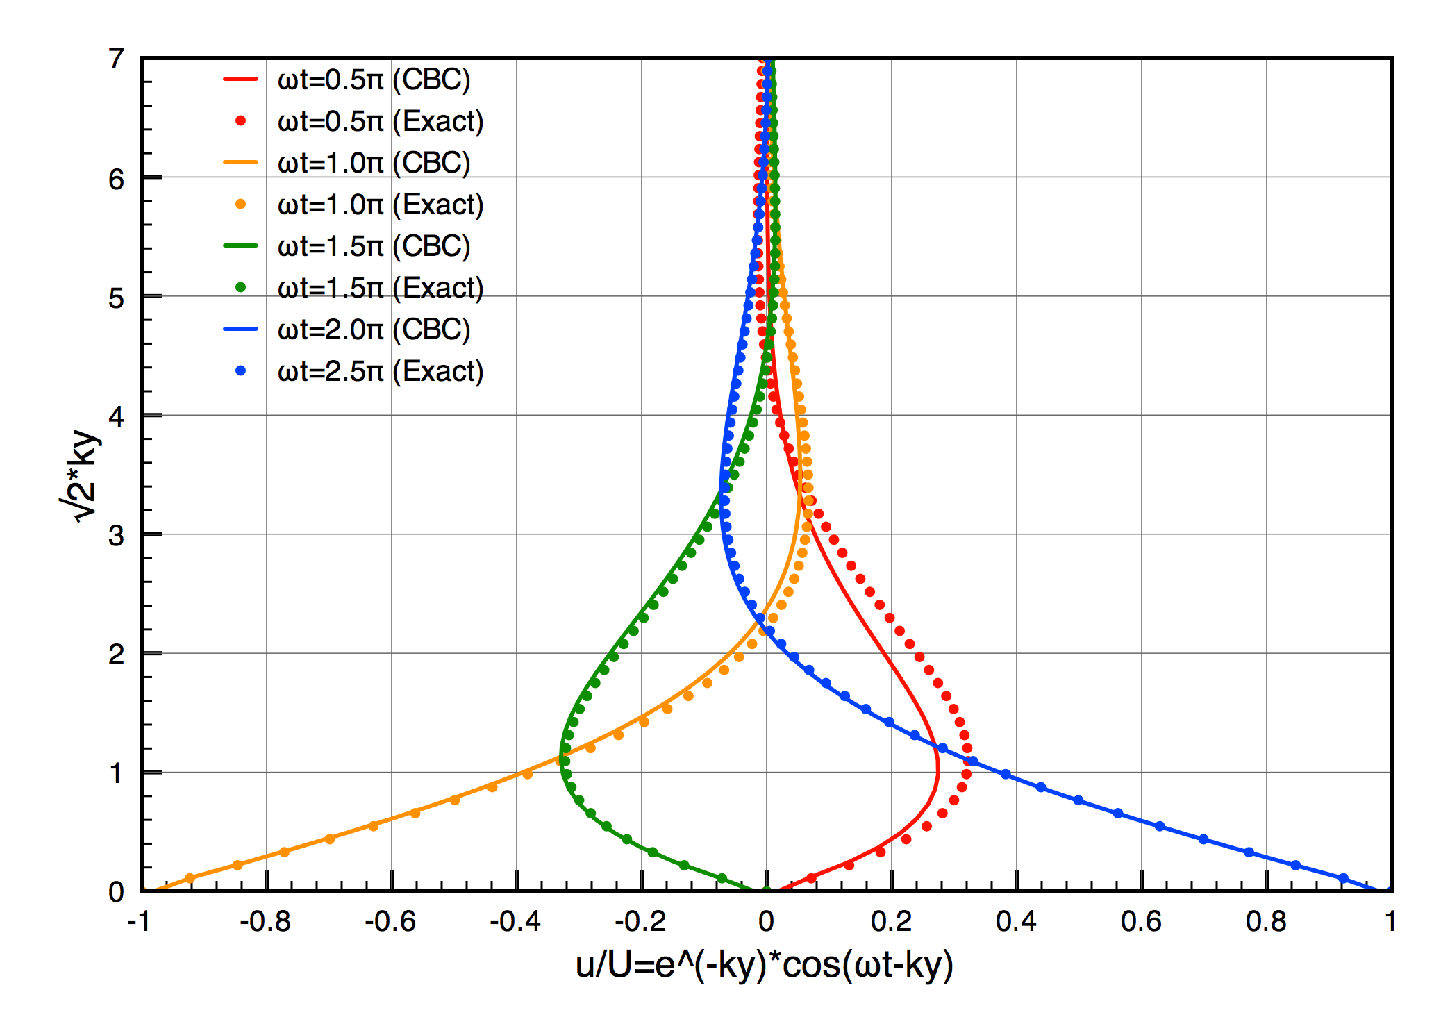
\includegraphics[width=14cm]{13-1stokes.eps}
\caption{Stokesの振動流の計算結果と厳密解の比較(計算1周期目)}
\label{fig:stokes_hikaku1}
%\end{figure}
%\begin{figure}[htbp]
%\centering
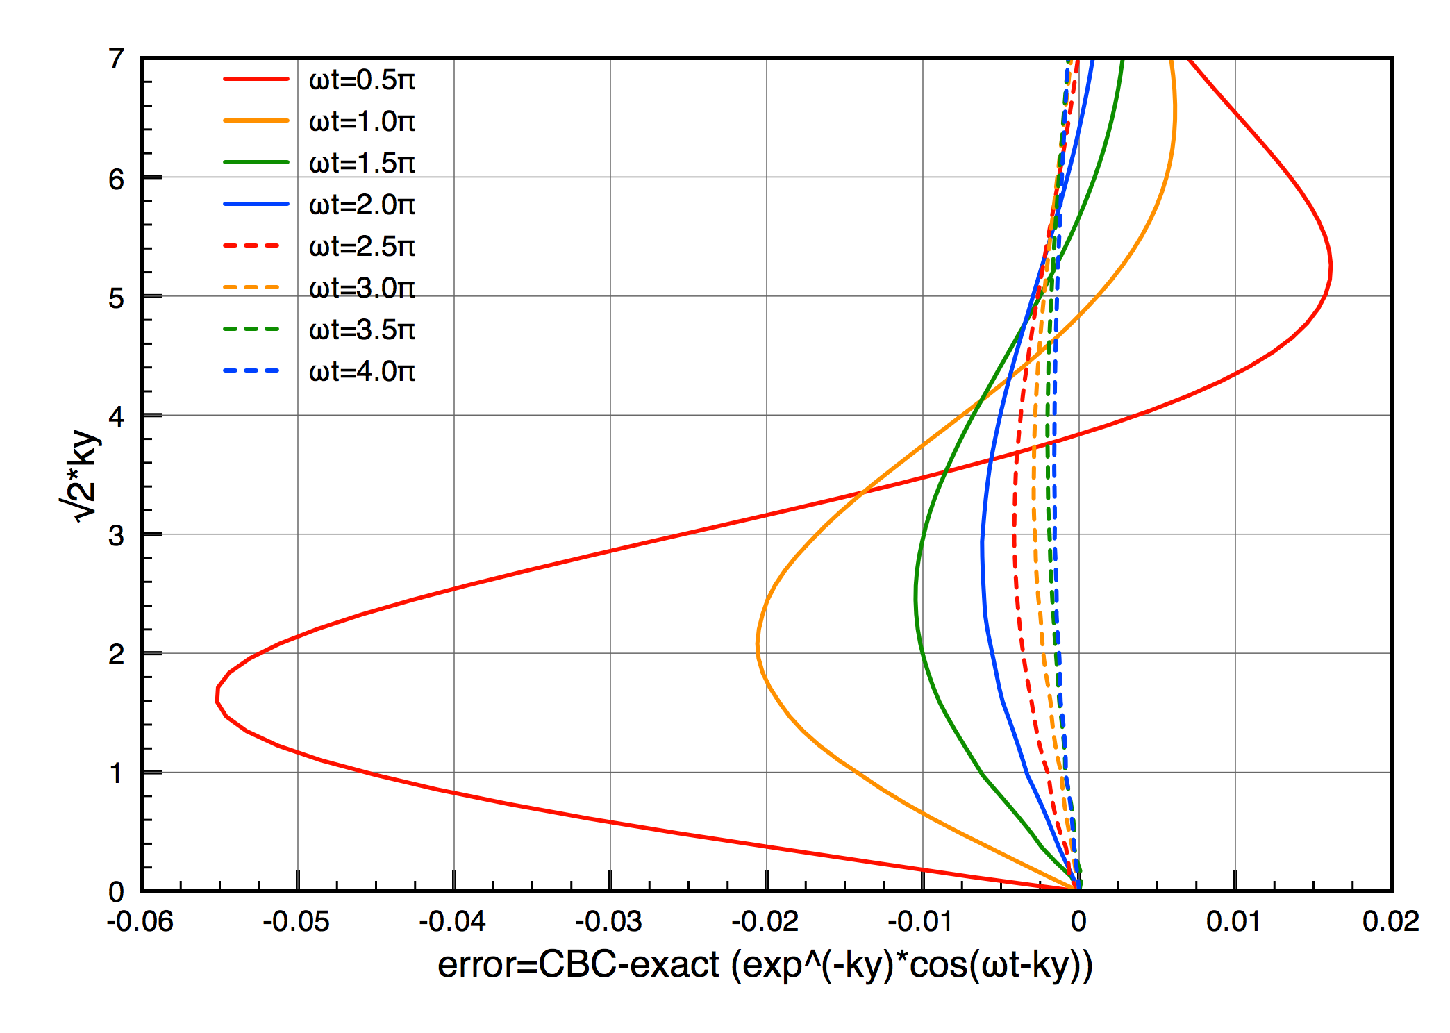
\includegraphics[width=14cm]{error1-2cycle.eps}
\caption{Stokesの振動流の計算結果の厳密解からの誤差}
\end{center}
\label{fig:stokes_error}
\end{figure}

\subsubsection{ファイルのメモ}
例題の提供ファイルの説明を以下に示す.
\begin{quote}
\begin{tabbing}
\hspace{15em}\= \hspace{20em}\kill
stokes.xml\> コンフィギュレーションXMLファイル\\
condition.txt \> 計算開始時conditionファイル\\
DomainInfo.txt \> 計算領域情報ファイル\\
history\_base.log.zip \> 履歴ファイル(解凍時3.5MB)\\
profiling.txt \> 実行性能測定結果ファイル\\
sample\_x=0\_y.log \> x=0上y軸に沿ったサンプリングファイル\\
plotフォルダ\> \textbf{図\ref{fig:stokes_exact}}〜\textbf{図\ref{fig:stokes_error}}のPlotファイルを含むフォルダ\\
\>(\url{http://plot/micw.eu/})\\
stokes2ndQ.mov.zip\> t=0[-]から56[-]までの$x=0$における$u$ベクトルのムービー(解凍時1MB).\\
\>元データは計算により出力されるvel***.sphファイル.\\
\>Visio(\url{http://vcad-hpsv.riken.jp/})で可視化できる.\\
gosa.f90\>sample\_x=0\_y.logを読み込み,厳密解からのエラーを算出するFortranプログラム
\end{tabbing}
\end{quote}

